\documentclass[11pt]{article}

\usepackage{fontspec}
\usepackage[margin=1in]{geometry}
\usepackage{amsmath}
\usepackage{array}
\usepackage{booktabs}
\usepackage{xcolor}
\usepackage{listings}
\usepackage{needspace}
\usepackage{tikz}
\usetikzlibrary{arrows.meta,positioning}
\usepackage[hidelinks]{hyperref}

\lstdefinelanguage{Rust}{
    morekeywords={
        as,async,await,break,const,continue,crate,else,enum,extern,false,fn,for,if,impl,in,let,loop,match,mod,move,mut,pub,ref,return,self,Self,static,struct,super,trait,true,type,unsafe,use,where,while,
        Some,None,Option,Either,Left,Right,Pubkey,Signature,Ctx8,u8,u16,u32,u256,bool
    },
    sensitive=true,
    morecomment=[l]{//},
    morestring=[b]"
}

\lstset{
    basicstyle=\ttfamily\footnotesize,
    breaklines=true,
    breakatwhitespace=true,
    columns=fullflexible,
    frame=single,
    framerule=0.25pt,
    rulecolor=\color{black!55},
    framesep=6pt,
    xleftmargin=1.4em,
    xrightmargin=1.4em,
    aboveskip=0.75\baselineskip,
    belowskip=0.75\baselineskip,
    keepspaces=true,
    keywordstyle=\color{blue!65!black}\bfseries,
    commentstyle=\color{green!45!black},
    stringstyle=\color{orange!60!black},
    emph={assert},
    emphstyle=\color{red!65!black}\bfseries,
    language=Rust,
    showstringspaces=false
}

% Byte-layout boxes for the wire-format figures. Widths are not to scale.
\tikzset{
    field/.style={draw, minimum height=2.6em, align=center,
    font=\ttfamily\scriptsize, inner sep=3pt, outer sep=0pt},
    rowlabel/.style={font=\footnotesize\itshape, anchor=west},
    bytecount/.style={font=\scriptsize, anchor=north},
}

% Absorb overfull boxes in prose that carries long typewriter identifiers.
\emergencystretch=4em

\title{Simplicity Multisig v0.1}

\author{
    Kyrylo Riabov\\
    \href{mailto:kyryl.ryabov@gmail.com}{\texttt{kyryl.ryabov@gmail.com}}
    \and
    Artem Chystiakov\\
    \href{mailto:artem.ch31@gmail.com}{\texttt{artem.ch31@gmail.com}}
}

\date{July 2026}

\begin{document}

    \maketitle

    \begin{abstract}
        We propose a practical and permissionless M-of-N multisig protocol that utilizes on-chain communication for the exchange of messages and signed intents between the signers. The described protocol leverages Simplicity language to allow multisig users to supplement their approval signatures with custom compliance and policy covenants without requiring a third-party service or authority. The proposed multisig can be implemented on Liquid and, in the future, on Bitcoin, once and if Simplicity becomes available there.
    \end{abstract}


    \section{Introduction}

    In today's Bitcoin ecosystem, multisigs are one of the most widely-used and critical logical structures, from the
    \texttt{OP\_CHECKMULTISIG} opcode \cite{bip11} and deterministic P2SH multisig addresses \cite{bip67}, to the Taproot script validation rules \cite{bip341,bip342}, MuSig2 \cite{musig2}, and FROST \cite{frost}. However, managing a multisig wallet generally assumes that participants have access to some communication channel. Signatures or partially signed transactions are expected to be exchanged through a coordination server, chat, or other out-of-band medium. Each of these dependencies must remain available whenever the funds need to move.

    Our goal is to reduce the dependencies that participants need in order to communicate. In the protocol proposed here, the whole setup consists of gathering the participants' public keys and descriptors and agreeing on a threshold. Once this is done, the multisig is ready to be used. After setup, the only communication layer that we assume is the blockchain itself, maximizing the reliability and availability of the coordination channel.

    The protocol defines how and under what conditions the multisig funds are spent. With the introduction of Simplicity on Liquid \cite{simplicity,liquid}, we are now able to introspect transactions in much greater detail compared to the regular Bitcoin Script.

    Using Simplicity, participants can aid their approval signatures with custom compliance and policy covenants that impose certain checks and conditions on the transaction structure, without requiring a third-party authority. Inside the script, a participant can enforce whitelists or blacklists of destinations, veto certain decisions, or attach a time constraint so that a signature given today can only be spent tomorrow and onward. Multisig schemes mentioned above cannot enforce such a promise. Once a signature is handed over, nothing prevents it from being used immediately.


    \section{On-Chain Coordination}
    \label{sec:coordination}

    \subsection{Participant Discovery}
    \label{sec:discovery}

    Multisig setup occurs out of band. Participants agree on an ordered list of x-only public keys and a threshold -- the number of approvals required to spend the multisig. This configuration determines the Taproot multisig address; Appendix~\ref{app:construction} describes its construction.

    After multisig setup, every vote a participant broadcasts must be discoverable by the other participants. For that purpose, we utilize descriptors \cite{bip380}.

    When participants confirm joining the multisig, each participant announces their own descriptor alongside the confirmation. Concretely, the participant makes a dust transfer to the multisig address and attaches \texttt{OP\_RETURN} outputs carrying an announcement record \cite{native-multisig-announcement}. The confirmation payload contains the participant's index in the ordered key list, x-only public key, descriptor, and a BIP-340 signature over a message that commits to the agreed threshold:

    \begin{equation}
        \mathrm{SHA256}(
        \texttt{"SIMPANNOUNCE-V1"}
        \,\|\, \mathrm{multisig\_script\_pubkey}
        \,\|\, \mathrm{index}
        \,\|\, \mathrm{pubkey}
        \,\|\, \mathrm{threshold}
        \,\|\, \mathrm{descriptor}
        ).
    \end{equation}

    The signature binds the descriptor to this exact multisig configuration, so the confirmation can neither be forged by a non-participant nor replayed against a different multisig. Announced descriptors must be public, and descriptors carrying blinding material MUST not be shared due to confidentiality reasons. Each participant announces exactly one descriptor. Conflicting announcements for one participant invalidate the multisig session. The scanner does not select a winner (Section~\ref{sec:limitations}).

    We additionally require that every vote published by a multisig participant be broadcast from this announced descriptor. This is what allows the discovery of votes and signed intent proposals. Scanning the multisig address yields the descriptors, and scanning the descriptors yields the votes.

    \subsection{Publishing Votes}
    \label{sec:votes}

    The core assumption of this step is that all vote scripts are known to every user. If a participant uses a custom policy covenant, its source file must be publicly available so that any other participant can compile it and reproduce the same executable leaf. We assume that all source files are publicly available and known to the users.

    With that in place, any participant can create a proposal. The participant selects multisig UTXOs, proposes the desired outputs, and signs the resulting message (Section~\ref{sec:compliance}). The vote is then created from the participant's announced descriptor as a single transaction that does two things:

    \begin{enumerate}
        \item It locks a dust amount to the vote covenant address. See  (Appendix~\ref{app:construction}) for more details about how the vote address is constructed;
        \item It attaches, in \texttt{OP\_RETURN} outputs, enough information for other participants to reconstruct the proposed transaction byte for byte and recompute the same signed message
        \cite{native-multisig-onchain-encoder}.
    \end{enumerate}

    Since the vote is published from an announced descriptor, it is trivially discoverable. A scanner walks the descriptors collected in Section~\ref{sec:discovery}, decodes every candidate transaction, recomputes the message hash, and verifies the embedded signature against the participant keys. Votes whose proposal inputs are already spent, or whose vote UTXO is spent, are discarded during scanning.

    \subsection{Wire Format}
    \label{sec:wire}

    Both multisig joining confirmation announcements (magic \texttt{SIMPANNC}) and vote proposals (magic \texttt{SIMPVOTE}) use the same chunked record framing. Every record is a single \texttt{OP\_RETURN} output whose script carries one data push of at most 75 bytes. Each record starts with a 10-byte header: an 8-byte magic, a 1-byte version (currently~1), and a 1-byte record kind.

    The payload that does not fit into one record is split into chunks of at most 63 bytes. Chunks are packed back to back without padding. Only the final chunk may be shorter. A metadata record announces how many chunks to expect, the total payload length, and a SHA-256 checksum of the reassembled payload. For vote proposals, the participant's signature travels in its own fixed-size record, so an executor can recover the proposal and the signature independently.

    Figure~\ref{fig:vote-records} shows the three vote record layouts, and Figure~\ref{fig:annc-payload} shows the confirmation announcement record layouts together with its reassembled payload.

    \begin{figure}[ht]
        \centering
        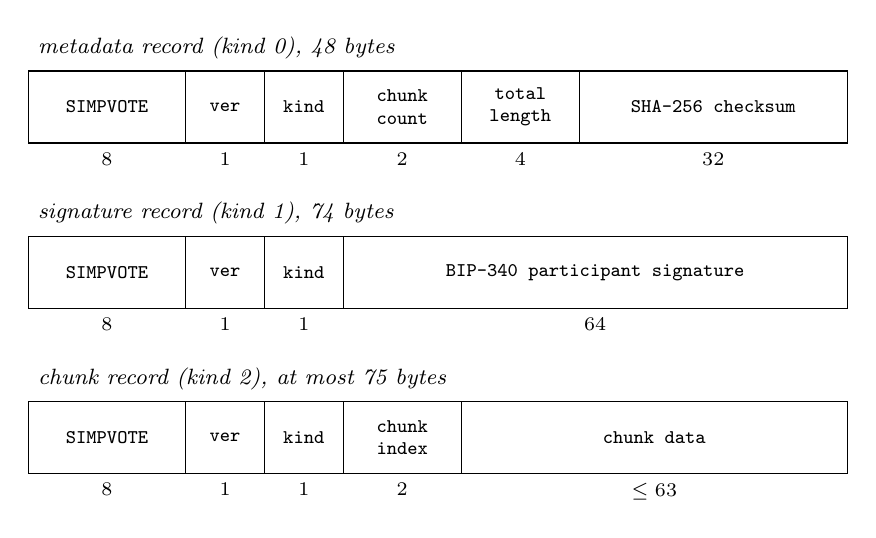
\begin{tikzpicture}[node distance=0pt]
            % --- metadata record ---
            \node[rowlabel] at (0,0.75) {metadata record (kind 0), 48 bytes};
            \node[field, minimum width=2.0cm, anchor=west] (m1) at (0,0) {SIMPVOTE};
            \node[field, minimum width=1.0cm, right=of m1] (m2) {ver};
            \node[field, minimum width=1.0cm, right=of m2] (m3) {kind};
            \node[field, minimum width=1.5cm, right=of m3] (m4) {chunk\\count};
            \node[field, minimum width=1.5cm, right=of m4] (m5) {total\\length};
            \node[field, minimum width=3.4cm, right=of m5] (m6) {SHA-256 checksum};
            \node[bytecount] at (m1.south) {8};
            \node[bytecount] at (m2.south) {1};
            \node[bytecount] at (m3.south) {1};
            \node[bytecount] at (m4.south) {2};
            \node[bytecount] at (m5.south) {4};
            \node[bytecount] at (m6.south) {32};
            % --- signature record ---
            \node[rowlabel] at (0,-1.35) {signature record (kind 1), 74 bytes};
            \node[field, minimum width=2.0cm, anchor=west] (s1) at (0,-2.1) {SIMPVOTE};
            \node[field, minimum width=1.0cm, right=of s1] (s2) {ver};
            \node[field, minimum width=1.0cm, right=of s2] (s3) {kind};
            \node[field, minimum width=6.4cm, right=of s3] (s4) {BIP-340 participant signature};
            \node[bytecount] at (s1.south) {8};
            \node[bytecount] at (s2.south) {1};
            \node[bytecount] at (s3.south) {1};
            \node[bytecount] at (s4.south) {64};
            % --- chunk record ---
            \node[rowlabel] at (0,-3.45) {chunk record (kind 2), at most 75 bytes};
            \node[field, minimum width=2.0cm, anchor=west] (c1) at (0,-4.2) {SIMPVOTE};
            \node[field, minimum width=1.0cm, right=of c1] (c2) {ver};
            \node[field, minimum width=1.0cm, right=of c2] (c3) {kind};
            \node[field, minimum width=1.5cm, right=of c3] (c4) {chunk\\index};
            \node[field, minimum width=4.9cm, right=of c4] (c5) {chunk data};
            \node[bytecount] at (c1.south) {8};
            \node[bytecount] at (c2.south) {1};
            \node[bytecount] at (c3.south) {1};
            \node[bytecount] at (c4.south) {2};
            \node[bytecount] at (c5.south) {$\le 63$};
        \end{tikzpicture}
        \caption{Vote proposal (\texttt{SIMPVOTE}) record layouts. Multi-byte integers are big-endian.}
        \label{fig:vote-records}
    \end{figure}

    \begin{figure}[ht]
        \centering
        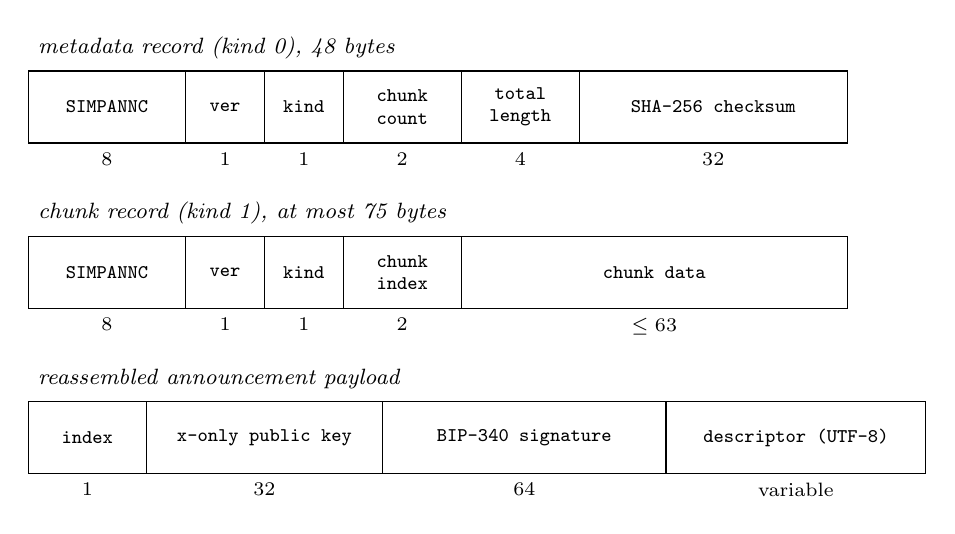
\begin{tikzpicture}[node distance=0pt]
            % --- metadata record ---
            \node[rowlabel] at (0,0.75) {metadata record (kind 0), 48 bytes};
            \node[field, minimum width=2.0cm, anchor=west] (m1) at (0,0) {SIMPANNC};
            \node[field, minimum width=1.0cm, right=of m1] (m2) {ver};
            \node[field, minimum width=1.0cm, right=of m2] (m3) {kind};
            \node[field, minimum width=1.5cm, right=of m3] (m4) {chunk\\count};
            \node[field, minimum width=1.5cm, right=of m4] (m5) {total\\length};
            \node[field, minimum width=3.4cm, right=of m5] (m6) {SHA-256 checksum};
            \node[bytecount] at (m1.south) {8};
            \node[bytecount] at (m2.south) {1};
            \node[bytecount] at (m3.south) {1};
            \node[bytecount] at (m4.south) {2};
            \node[bytecount] at (m5.south) {4};
            \node[bytecount] at (m6.south) {32};
            % --- chunk record ---
            \node[rowlabel] at (0,-1.35) {chunk record (kind 1), at most 75 bytes};
            \node[field, minimum width=2.0cm, anchor=west] (c1) at (0,-2.1) {SIMPANNC};
            \node[field, minimum width=1.0cm, right=of c1] (c2) {ver};
            \node[field, minimum width=1.0cm, right=of c2] (c3) {kind};
            \node[field, minimum width=1.5cm, right=of c3] (c4) {chunk\\index};
            \node[field, minimum width=4.9cm, right=of c4] (c5) {chunk data};
            \node[bytecount] at (c1.south) {8};
            \node[bytecount] at (c2.south) {1};
            \node[bytecount] at (c3.south) {1};
            \node[bytecount] at (c4.south) {2};
            \node[bytecount] at (c5.south) {$\le 63$};
            % --- reassembled payload ---
            \node[rowlabel] at (0,-3.45) {reassembled announcement payload};
            \node[field, minimum width=1.5cm, anchor=west] (p1) at (0,-4.2) {index};
            \node[field, minimum width=3.0cm, right=of p1] (p2) {x-only public key};
            \node[field, minimum width=3.6cm, right=of p2] (p3) {BIP-340 signature};
            \node[field, minimum width=3.3cm, right=of p3] (p4) {descriptor (UTF-8)};
            \node[bytecount] at (p1.south) {1};
            \node[bytecount] at (p2.south) {32};
            \node[bytecount] at (p3.south) {64};
            \node[bytecount] at (p4.south) {variable};
        \end{tikzpicture}
        \caption{Participant announcement (\texttt{SIMPANNC}) record layouts and reassembled payload.}
        \label{fig:annc-payload}
    \end{figure}

    For vote proposals, the encoded payload (chunk data) is the fully serialized proposal transaction. Decoding therefore reconstructs the exact transaction shape, and recomputing the base message over it (Appendix~\ref{app:message}) yields the same hash the participant signed. Figure~\ref{fig:chunking} visualizes the encoding of one proposal.

    A decoder accepts a transaction only if all of the following hold: there is exactly one metadata record (for votes, exactly one signature record), no chunk index is duplicated or out of bounds, every chunk is present, the concatenated length equals the announced total length, and the SHA-256 checksum matches. Anything else is rejected, so a malformed or partially confirmed carrier transaction can never produce a plausible-looking proposal.

    \paragraph{Relay Policy.}
    Each record occupies a separate output, so a carrier transaction uses multiple \texttt{OP\_RETURN} outputs, each with a scriptPubKey of at most 77 bytes. Liquid relay policy permits this layout. Elements allows multiple data-carrier outputs on PAK-enforced chains, including Liquid mainnet (\texttt{multi\_data\_permitted}),
    and each output remains below the default 83-byte limit \cite{elements-policy}. Bitcoin relay policy historically allowed only one \texttt{OP\_RETURN} output per transaction. However,
    Bitcoin Core~30.0 instead applies the data-carrier limit to their combined size \cite{bitcoin-core-30}.

    \paragraph{Current limitation.}
    The protocol currently supports only unconfidential transactions on Liquid. Confidential transport would require exchanging blinding material between participants, encrypting the carried payload, and carrying substantially larger data in a medium where every byte is paid for. We consider this a natural follow-up work and keep it out of scope in this version.

    \begin{figure}[ht]
        \centering
        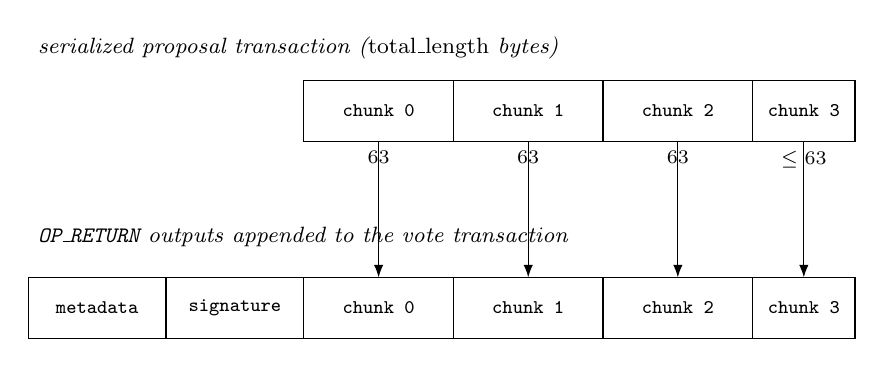
\begin{tikzpicture}[
            >={Latex[length=1.6mm]},
            chunkbox/.style={draw, minimum height=2.2em, align=center,
            font=\ttfamily\scriptsize, inner sep=3pt, outer sep=0pt},
            node distance=0pt
        ]
            % payload bar
            \node[rowlabel] at (0,0.8) {serialized proposal transaction ($\mathrm{total\_length}$ bytes)};
            \node[chunkbox, minimum width=1.9cm, anchor=west] (t1) at (3.5,0) {chunk 0};
            \node[chunkbox, minimum width=1.9cm, right=of t1] (t2) {chunk 1};
            \node[chunkbox, minimum width=1.9cm, right=of t2] (t3) {chunk 2};
            \node[chunkbox, minimum width=1.3cm, right=of t3] (t4) {chunk 3};
            \node[bytecount] at (t1.south) {63};
            \node[bytecount] at (t2.south) {63};
            \node[bytecount] at (t3.south) {63};
            \node[bytecount] at (t4.south) {$\le 63$};
            % outputs
            \node[rowlabel] at (0,-1.6) {\texttt{OP\_RETURN} outputs appended to the vote transaction};
            \node[chunkbox, minimum width=1.75cm, anchor=west] (o0) at (0,-2.5) {metadata};
            \node[chunkbox, minimum width=1.75cm, right=of o0] (o1) {signature};
            \node[chunkbox, minimum width=1.9cm, right=of o1] (o2) {chunk 0};
            \node[chunkbox, minimum width=1.9cm, right=of o2] (o3) {chunk 1};
            \node[chunkbox, minimum width=1.9cm, right=of o3] (o4) {chunk 2};
            \node[chunkbox, minimum width=1.3cm, right=of o4] (o5) {chunk 3};
            % arrows
            \draw[->] (t1.south) -- (o2.north);
            \draw[->] (t2.south) -- (o3.north);
            \draw[->] (t3.south) -- (o4.north);
            \draw[->] (t4.south) -- (o5.north);
        \end{tikzpicture}
        \caption{Encoding a vote proposal into chunked \texttt{OP\_RETURN} outputs. Chunks are packed without padding; only the final chunk may be shorter.}
        \label{fig:chunking}
    \end{figure}

    \subsection{Happy Path: a 2-of-3 Walkthrough}
    \label{sec:happy-path}

    Figure~\ref{fig:sequence} assembles the pieces into the full happy flow of a 2-of-3 multisig, from creation to spend. Alice, Bob, and Carol perform the one-time setup. Alice proposes a spend, Bob agrees, and Alice executes it. No message other than a Liquid transaction is exchanged after setup.

    The final spend follows the transaction shape enforced by the covenants and exercised by the regtest scenarios \cite{native-multisig-regtest}: multisig inputs occupy the input prefix starting at index zero, vote inputs come directly after the multisig input window, and proposed outputs start at output index zero, followed by the fee. The dust amounts held by the vote UTXOs are used as the transaction fee \cite{native-multisig-spend}.


    \section{Covenant-Enforced Compliance}
    \label{sec:compliance}

    The multisig itself is a Simplicity covenant \cite{native-multisig-multisig}, and each approval is a \emph{vote}.

    A participant does not sign a whole transaction. Instead, the participant signs the transaction shape that includes the multisig inputs and the proposed outputs, that are bound to the hash of the executable policy leaf (vote covenant).

    The multisig covenant reconstructs the vote Taproot tree from the vote leaf hash and the signature, and asserts that an input with exactly this script is present in the spending transaction. If the policies are changed, signature verification fails.

    The executable leaf can contain any check that Simplicity can express: whitelist and blacklist checks on destination scripts, amount limits, compliance rules, pay-to-use conditions, or a timelock that makes the signature valid only from tomorrow onward.

    The message construction, the vote Taproot tree, threshold checks, input and output windows, and the handling of uncounted vote inputs, together with the corresponding code snippets and security considerations are given in Appendix~\ref{app:construction}.

    \begin{figure}[p]
        \centering
        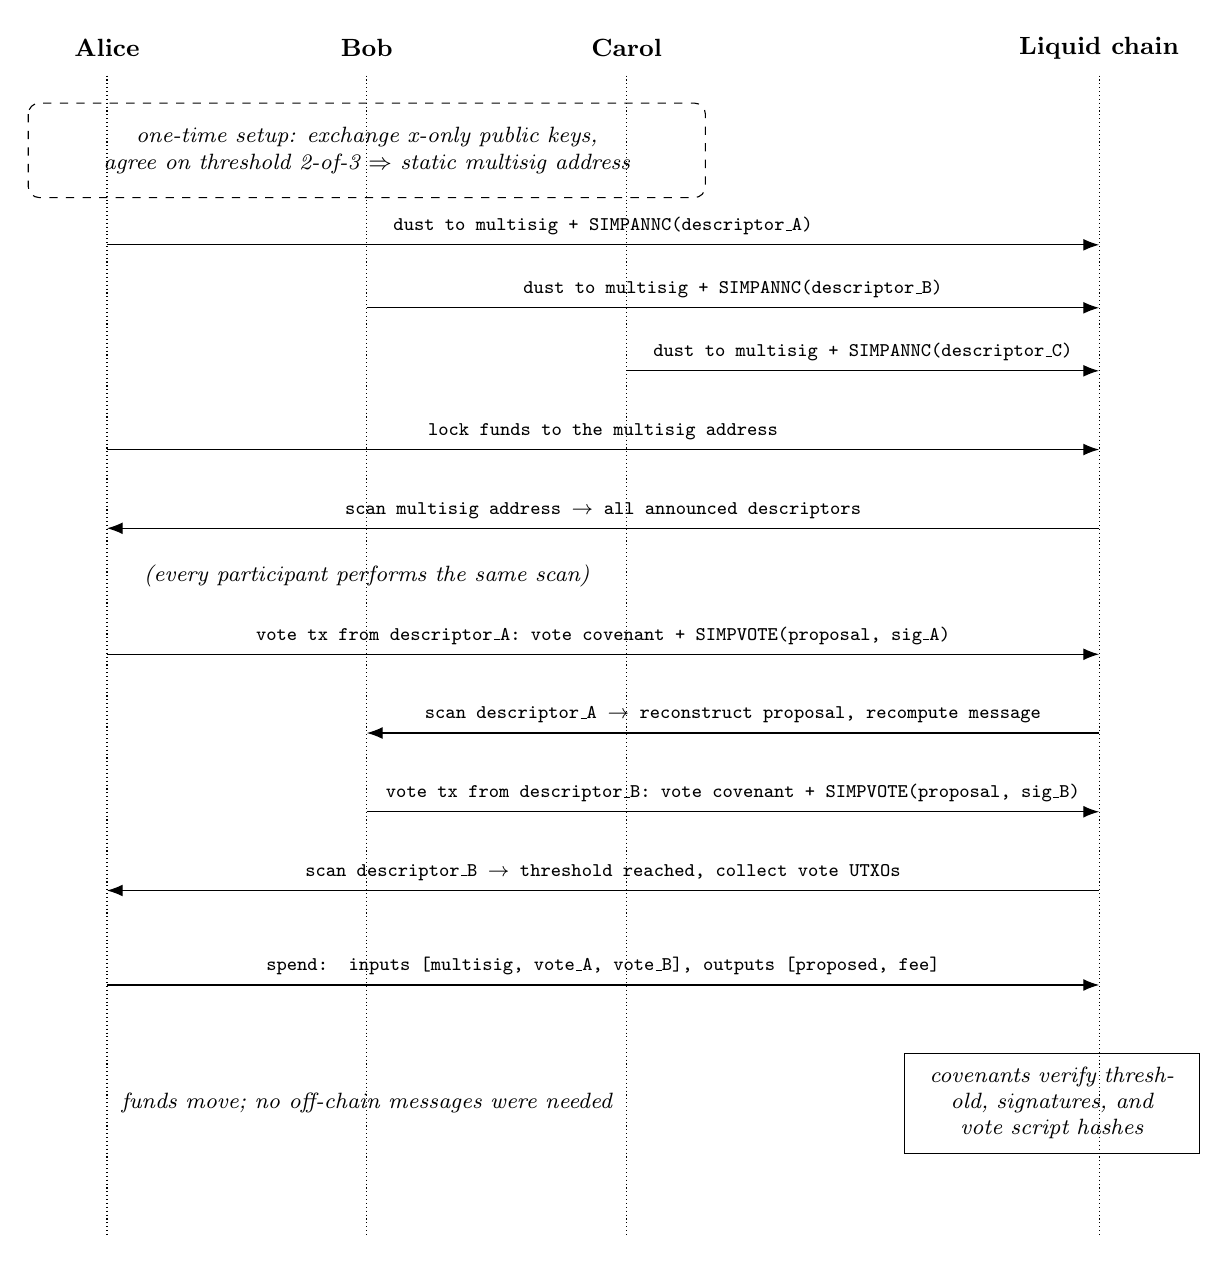
\begin{tikzpicture}[
            >={Latex[length=2mm]},
            msg/.style={font=\scriptsize\ttfamily},
            note/.style={font=\footnotesize\itshape, align=center},
            actor/.style={font=\bfseries\small}
        ]
            \def\A{0} \def\B{3.3} \def\C{6.6} \def\L{12.6}
            % actors
            \node[actor] at (\A,0) {Alice};
            \node[actor] at (\B,0) {Bob};
            \node[actor] at (\C,0) {Carol};
            \node[actor] at (\L,0) {Liquid chain};
            % lifelines
            \foreach \x in {\A,\B,\C,\L} \draw[densely dotted] (\x,-0.35) -- (\x,-15.1);
            % setup box
            \draw[dashed, rounded corners] (\A-1.0,-0.7) rectangle (\C+1.0,-1.9);
            \node[note] at (\C/2,-1.3)
                {one-time setup: exchange x-only public keys,\\
            agree on threshold 2-of-3 $\Rightarrow$ static multisig address};
            % announcements
            \draw[->] (\A,-2.5) -- (\L,-2.5)
            node[midway, above, msg] {dust to multisig + SIMPANNC(descriptor\_A)};
            \draw[->] (\B,-3.3) -- (\L,-3.3)
            node[midway, above, msg] {dust to multisig + SIMPANNC(descriptor\_B)};
            \draw[->] (\C,-4.1) -- (\L,-4.1)
            node[midway, above, msg] {dust to multisig + SIMPANNC(descriptor\_C)};
            % funding
            \draw[->] (\A,-5.1) -- (\L,-5.1)
            node[midway, above, msg] {lock funds to the multisig address};
            % discovery
            \draw[<-] (\A,-6.1) -- (\L,-6.1)
            node[midway, above, msg] {scan multisig address $\rightarrow$ all announced descriptors};
            \node[note] at (\C/2,-6.7) {(every participant performs the same scan)};
            % proposal
            \draw[->] (\A,-7.7) -- (\L,-7.7)
            node[midway, above, msg]
                {vote tx from descriptor\_A: vote covenant + SIMPVOTE(proposal, sig\_A)};
            \draw[<-] (\B,-8.7) -- (\L,-8.7)
            node[midway, above, msg]
                {scan descriptor\_A $\rightarrow$ reconstruct proposal, recompute message};
            \draw[->] (\B,-9.7) -- (\L,-9.7)
            node[midway, above, msg]
                {vote tx from descriptor\_B: vote covenant + SIMPVOTE(proposal, sig\_B)};
            \draw[<-] (\A,-10.7) -- (\L,-10.7)
            node[midway, above, msg]
                {scan descriptor\_B $\rightarrow$ threshold reached, collect vote UTXOs};
            % final spend
            \draw[->] (\A,-11.9) -- (\L,-11.9)
            node[midway, above, msg]
                {spend: inputs [multisig, vote\_A, vote\_B], outputs [proposed, fee]};
            % verification note
            \node[note, draw, text width=3.4cm, inner sep=5pt] at (\L-0.6,-13.4)
                {covenants verify threshold, signatures, and vote script hashes};
            \node[note] at (\C/2,-13.4) {funds move; no off-chain messages were needed};
        \end{tikzpicture}
        \caption{Happy flow of a 2-of-3 multisig: creation, announcements, proposal, second vote, and the final spend. After the one-time setup, every arrow is a Liquid transaction or a chain scan.}
        \label{fig:sequence}
    \end{figure}


    \section{Bitcoin Compatibility}

    Even though the multisig is based on Simplicity, there is ongoing work to add Simplicity to Bitcoin Inquisition \cite{bitcoin-inquisition-binana-simplicity,bitcoin-inquisition-simplicity-impl}.

    All core jets that were used in the current multisig are present in the Bitcoin version as well. Therefore, this solution is Bitcoin-compatible if Simplicity is ever added to Bitcoin itself.


    \section{Formal Verification}

    The work on formal verification of the multisig covenants is ongoing. Details will be mentioned separately when it is done.


    \section{Limitations and Future Work}
    \label{sec:limitations}

    \paragraph{Privacy.}
    Public descriptors link each vote to its participant, and publishing a descriptor on-chain permanently exposes the transaction history it covers. This enables permissionless discovery but sacrifices privacy. Confidential coordination, like confidential transport (Section~\ref{sec:wire}), remains out of scope.

    \paragraph{Descriptor rotation.}
    The protocol does not support descriptor rotation. Changing a descriptor requires a new multisig setup. Conflicting announcements for one participant invalidate the session. The reference implementation gives priority to neither the first nor the last.

    \paragraph{Encrypted coordination.}
    The protocol does not currently hide vote contents from outside observers. A future version could establish a group secret during setup and use it to derive per-participant tag chains and encrypt payloads, following BIP-352 \cite{bip352}. It could also derive a view key for a designated auditor.

    \paragraph{Policy source distribution.}
    Custom policy sources (vote covenants) must remain publicly available (Section~\ref{sec:votes}), leaving one off-chain dependency. A future version could commit to sources on chain or distribute them through content-addressed storage.

    \appendix


    \section{Multisig Construction and Security Considerations}
    \label{app:construction}

    This appendix contains the full construction of the Simplicity multisig and its security considerations, including the relevant code snippets from the reference implementation.

    \subsection{Message Construction}
    \label{app:message}

    The most sensitive part is the message that is signed by every participant.

    In the reference version of the multisig \cite{native-multisig-multisig}, the message that is verified by users includes:

    \begin{enumerate}
        \item \texttt{jet::input\_hash(0..=i)} \cite{simplicity-input-hash}, where $i$ is the last multisig input;
        \item \texttt{jet::output\_hash(0..=j)} \cite{simplicity-output-hash}, where $j$ is the last desired output;
        \item Policies that must be validated before allowing the use of the signature.
    \end{enumerate}

    \textbf{Important note:} in this model, only a part of the transaction is signed. Therefore, when a participant creates the message, they must ensure that, for example, when 1 LBTC is spent, all outputs that should be constrained are in the range $0..=j$. Before signing, a participant MUST verify, for each asset, that the sum of the committed multisig input amounts equals the sum of the proposed output amounts in the signed range plus the amounts of any declared fee outputs. Otherwise, the signature leaves the remainder unconstrained. The reference implementation enforces this check both when a proposal is created and when a vote is signed.

    Enforcing this per-asset balance check in the multisig covenant is out of scope for this paper.

    As a result, the base message is:

    \begin{equation}
        \mathrm{base\_message}
        =
        \mathrm{SHA256}(
        t_{\mathrm{base}}
        \,\|\,
        t_{\mathrm{base}}
        \,\|\,
        \mathrm{input\_hashes}
        \,\|\,
        \mathrm{output\_hashes}
        ),
    \end{equation}

    where $t_{\mathrm{base}} = \mathrm{SHA256}(\texttt{"SIMPVOTE-BASE-V1"})$. Prefixing the payload with two copies of the ASCII tag hash follows the BIP-340 tagged-hash construction and separates this message from other protocol contexts.

    Every participant signs a message that also contains the executable leaf hash, which represents the set of their policies:

    \begin{equation}
        \mathrm{participant\_message}
        =
        \mathrm{SHA256}(
        t_{\mathrm{msg}}
        \,\|\,
        t_{\mathrm{msg}}
        \,\|\,
        \mathrm{vote\_executable\_leaf\_hash}
        \,\|\,
        \mathrm{base\_message}
        ),
    \end{equation}

    where $t_{\mathrm{msg}} = \mathrm{SHA256}(\texttt{"SIMPVOTE-MSG-V1"})$.

    \subsection{Programmable Signature}

    Below is a diagram of a Taproot tree, which generally represents a Taproot output that includes Simplicity with stateful TapData \cite{bip341,simplicity-state}.

    \begin{figure}[ht]
        \centering
        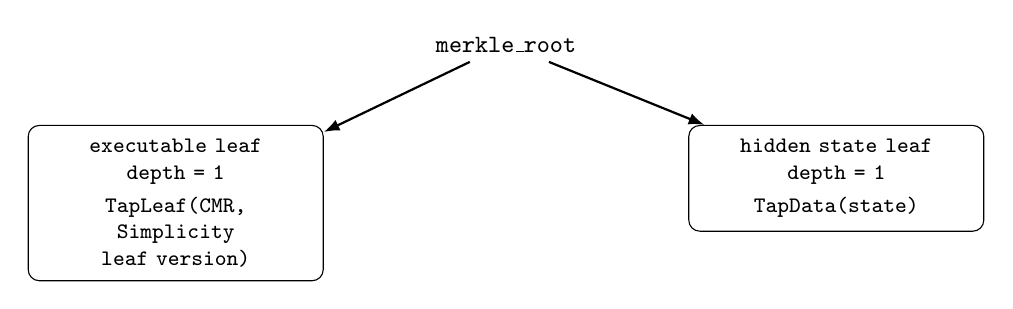
\begin{tikzpicture}[
            node distance=0.8cm and 1.3cm,
            root/.style={font=\ttfamily\small},
            box/.style={draw, rounded corners, align=center, font=\ttfamily\footnotesize,
            inner sep=5pt, text width=0.28\linewidth},
            arrow/.style={-{Latex[length=2mm]}, thick}
        ]
            \node[root] (root) {merkle\_root};
            \node[box, below left=of root] (exec) {
                executable leaf\\
                depth = 1\\[0.3em]
                TapLeaf(CMR,\\
                Simplicity leaf version)
            };
            \node[box, below right=of root] (state) {
                hidden state leaf\\
                depth = 1\\[0.3em]
                TapData(state)
            };

            \draw[arrow] (root) -- (exec);
            \draw[arrow] (root) -- (state);
        \end{tikzpicture}
        \caption{Vote Taproot tree with executable Simplicity leaf and hidden TapData state.}
    \end{figure}

    The hidden state leaf commits to the participant signature as follows:

    \begin{equation}
        \begin{aligned}
            \mathrm{TapData(state)}
            = \mathrm{SHA256}(&
            \mathrm{SHA256}(\texttt{"TapData"}) \,\|\, \\
            &
            \mathrm{SHA256}(\texttt{"TapData"}) \,\|\, \\
            &
            \mathrm{SHA256}(\mathrm{participant\_signature})
            ).
        \end{aligned}
    \end{equation}

    The executable leaf (vote) is the left branch of the tree. This branch contains all the Simplicity checks of the vote, for example enforcing that one of the outputs sends Dave 0.1 BTC.

    Simplicity's Taproot integration is described in the Simplicity Taproot work
    \cite{simplicity-taproot-universal-sighashes}.

    The implementation of the vote contract is in \texttt{vote.simf} \cite{native-multisig-vote}.

    The right branch contains the signature part. This branch is checked by the multisig covenant to verify that the correct ``vote'' was included
    \cite{native-multisig-multisig}.

    Due to the UTXO nature of Liquid, every vote will contain either a dust amount of LBTC or a throwaway token. The way the vote is created and discovered on-chain is described in Section~\ref{sec:coordination}.

    \subsection{Threshold Checks}

    The provided reference implementation of the multisig \cite{native-multisig-multisig} includes the basic n-of-3 check. This means that three users can gather together and agree on the desired threshold.

    If a bigger number of participants is expected, a contract modification is required due to compiler constraints. At the time of writing this paper, SimplicityHL does not allow parameterizing the size of the array.

    \Needspace{7\baselineskip}
    The sanity checks of the threshold parameter are as follows:

    \begin{lstlisting}
let threshold: u32 = param::THRESHOLD;
// Sanity checks to ensure that the multisig is spendable.
assert!(jet::le_32(1, threshold));
assert!(jet::le_32(threshold, 3));
    \end{lstlisting}

    \Needspace{12\baselineskip}
    and:

    \begin{lstlisting}
// Verification is done in the following order.
// Starting after the multisig inputs, if the signature for input i is None, skip it.
// Otherwise, calculate the expected vote script hash and check that it matches.
// Then check the signature against participants[i].
// This action is performed for all participants.
// Finally, check that the number of non-None signatures is >= the threshold.
let (valid_votes, next_vote_input_index): (u32, u32) =
  count_votes(participants, votes, multisig_input_count, base_message);
assert!(jet::le_32(threshold, valid_votes));
    \end{lstlisting}

    With the last check, we iterate over provided user inputs. It means that to spend the multisig input, it should have, for example, at least two votes if the threshold is two.

    This constraint is related to the following check:

    \begin{lstlisting}
// We need to ensure that during spending we have enough votes.
let (carry, minimum_inputs_num): (bool, u32) =
  jet::add_32(threshold, multisig_input_count);
ensure_zero_bit(carry);
assert!(jet::le_32(minimum_inputs_num, jet::num_inputs()));
    \end{lstlisting}

    This checks that the transaction has enough inputs to actually spend the multisig. The logic is that, for example, to spend a 2-of-3 multisig, you need at least three inputs: one for the multisig and two for the vote covenants.

    \subsection{Multisig Input and Output Windows}

    Every multisig input is signed.

    \begin{lstlisting}
// For every vote entry, verify the presence of the on-chain commitment
// and the correctness of the signed message.
fn count_vote_entry(
  entry: (Pubkey, Option<(Signature, u256)>),
  acc: (u32, u32, u256)
) -> (u32, u32, u256) {
  let (participant, maybe_vote): (Pubkey, Option<(Signature, u256)>) = entry;
  let (valid_votes, next_vote_input_index, base_message): (u32, u32, u256) = acc;

  let (valid_votes, next_vote_input_index): (u32, u32) = match maybe_vote {
    Some(vote: (Signature, u256)) => {
      let (participant_signature, vote_executable_leaf_hash): (Signature, u256) = vote;

      verify_vote_input(next_vote_input_index, vote_executable_leaf_hash, participant_signature);
      checksig(participant, participant_signature, vote_executable_leaf_hash, base_message);

      (increment_checked(valid_votes), increment_checked(next_vote_input_index))
    }
    None => (valid_votes, next_vote_input_index),
  };

  (valid_votes, next_vote_input_index, base_message)
}
    \end{lstlisting}

    In the covenant, until we reach the last non-multisig input, we collect the signatures:

    \begin{lstlisting}
// Continue iterating over the inputs until the script hash no longer matches.
// This also enforces that multisig inputs start at index 0.
fn add_multisig_input_hash(acc: (Ctx8, u32), current_script_hash: u256, index: u8)
  -> Either<(Ctx8, u32), (Ctx8, u32)> {
  let (ctx, multisig_input_count): (Ctx8, u32) = acc;

  let index: u32 = jet::left_pad_low_8_32(index);
  let input_script_hash: Option<u256> = jet::input_script_hash(index);

  match input_script_hash {
    Some(input_script_hash: u256) => {
      match jet::eq_256(input_script_hash, current_script_hash) {
        true => {
          let next_ctx: Ctx8 =
            jet::sha_256_ctx_8_add_32(ctx, unwrap(jet::input_hash(index)));
          let next_multisig_input_count: u32 = increment_checked(multisig_input_count);
          Right((next_ctx, next_multisig_input_count))
        },
        false => Left((ctx, multisig_input_count)),
      }
    },
    None => Left((ctx, multisig_input_count)),
  }
}
    \end{lstlisting}

    The covenant verifies that if a multisig input is present, it is spent in the window from zero up to the last multisig input. The covenant also checks that the current multisig input is included in the signed base message:

    \begin{lstlisting}
let (base_message, multisig_input_count): (u256, u32) =
  base_message_and_input_count(witness::TOTAL_PROPOSED_OUTPUTS);
// Another sanity check: enforce that multisig covenant inputs start at index 0.
// This fails if the UTXO at index 0 is not a multisig.
assert!(jet::le_32(1, multisig_input_count));
// Ensure that the current multisig input is included in the signed base message.
assert!(jet::lt_32(jet::current_index(), multisig_input_count));
    \end{lstlisting}

    The second part that is included in the base message are the outputs:

    \begin{lstlisting}
// Build the base message that participants sign.
//
// The message signed by each participant includes all multisig inputs,
// i.e. jet::input_hash(i).
//
// It also includes outputs proposed by the participant,
// i.e. jet::output_hash(i).
fn base_message_and_input_count(total_proposed_outputs: u16) -> (u256, u32) {
  let ctx: Ctx8 = jet::sha_256_ctx_8_init();
  let input_result =
    for_while::<add_multisig_input_hash>((ctx, 0), jet::current_script_hash());

  let (ctx, multisig_input_count): (Ctx8, u32) = unwrap_left(input_result);
  let output_result = for_while::<add_proposed_output_hash>(ctx, total_proposed_outputs);

  let ctx: Ctx8 = unwrap_left(output_result);

  (jet::sha_256_ctx_8_finalize(ctx), multisig_input_count)
}
    \end{lstlisting}

    As shown above, in the final signature check we also append the
    \texttt{vote\_executable\_leaf\_hash}. This leads to the last check: vote execution checks.

    To check that the vote was included in the transaction, the multisig needs to check that an input with the desired policies is included.

    \begin{lstlisting}
// This function verifies that the proved signature is committed on-chain
// through the intended vote.simf program.
// The intended vote.simf program is the one signed by the participant.
fn verify_vote_input(
  input_index: u32,
  vote_executable_leaf_hash: u256,
  participant_signature: Signature
) {
  let state_hash_ctx1: Ctx8 = jet::sha_256_ctx_8_init();
  let state_hash_ctx2: Ctx8 =
    jet::sha_256_ctx_8_add_64(state_hash_ctx1, Signature::into(participant_signature));
  let state_hash: u256 = jet::sha_256_ctx_8_finalize(state_hash_ctx2);

  let tap_leaf: u256 = vote_executable_leaf_hash;
  let state_ctx1: Ctx8 = jet::tapdata_init();
  let state_ctx2: Ctx8 = jet::sha_256_ctx_8_add_32(state_ctx1, state_hash);
  let state_leaf: u256 = jet::sha_256_ctx_8_finalize(state_ctx2);
  let tap_node: u256 = jet::build_tapbranch(tap_leaf, state_leaf);

  let bip0341_key: u256 =
    0x50929b74c1a04954b78b4b6035e97a5e078a5a0f28ec96d547bfee9ace803ac0;
  let tweaked_key: u256 = jet::build_taptweak(bip0341_key, tap_node);

  let hash_ctx1: Ctx8 = jet::sha_256_ctx_8_init();
  let hash_ctx2: Ctx8 = jet::sha_256_ctx_8_add_2(hash_ctx1, 0x5120);
  let hash_ctx3: Ctx8 = jet::sha_256_ctx_8_add_32(hash_ctx2, tweaked_key);
  let expected_vote_script_hash: u256 = jet::sha_256_ctx_8_finalize(hash_ctx3);

  assert!(jet::eq_256(
    unwrap(jet::input_script_hash(input_index)),
    expected_vote_script_hash
  ));
}
    \end{lstlisting}

    To do that, we reconstruct the Merkle tree and perform the last assertion:

    \begin{lstlisting}
assert!(jet::eq_256(
  unwrap(jet::input_script_hash(input_index)),
  expected_vote_script_hash
));
    \end{lstlisting}

    This makes clear why the expected vote script hash is included in the message that is signed by the participant and how the multisig enforces a programmable check. If the policies are changed, the signature verification fails. Also, by Bitcoin consensus rules, when an input is included in the transaction that is being spent, the proper witness should be provided.

    \subsection{Uncounted Vote Inputs}
    \label{app:uncounted}

    There is a caveat on how uncounted votes can be spent; see \texttt{vote.simf} for more details \cite{native-multisig-vote}.

    In a nutshell, during a 1-of-3 multisig execution, all three votes can be provided, but only one of them is needed to be checked. From the multisig perspective, this is fine because the threshold is met. However, the value that the vote holds can be moved to any address if it is not constrained by the message that is signed. Dealing with this issue is out of scope of this paper.

    \bibliographystyle{unsrt}
    \bibliography{references}

\end{document}
